
% UC... specificare App o Server -> UCA / UCS


\section{UCS 1 - Autenticazione al Server}

\begin{figure}[h]
  \caption{Didascalia}
  \centering
    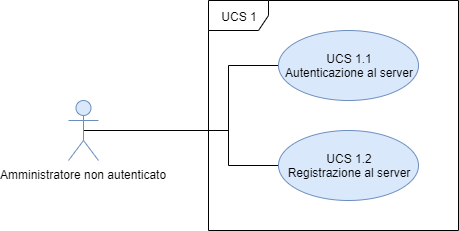
\includegraphics[scale=0.6]{sezioni/UseCase/Immagini/UCS1.png}
\end{figure}

\begin{itemize}
\item \textbf{Attori primari:} Amministratore non autenticato
\item \textbf{Precondizione:} L'amministratore non è autenticato
\item \textbf{Postcondizione:}  L'amministratore è stato autenticato e può avere accesso alle funzionalità offerte dal sistema
\item \textbf{Scenario principale:} Amministratore non identificato inserisce il nome utente e la password per autenticarsi al server 
\item \textbf{Flusso di eventi:}
    \begin{enumerate}
        \item UCS 1.1 - Inserimento e-mail;
        \item UCS 1.2 - Inserimento password;
        \item UCS 1.3 - Password dimenticata;
        
    \end{enumerate}
\item \textbf{Estensioni:}
	\begin{enumerate}		
		\item UCS 1.4 - Credenziali errate;
	\end{enumerate}
\end{itemize}


\subsection{UCS 1.1}%sea level
\begin{itemize}
\item \textbf{Nome:} Inserimento e-mail
\item \textbf{Attori primari:}  Utente non autenticato
%\item \textbf{Attori secondari:}%opzionale
\item \textbf{Precondizione:}  L'amministratore non è autenticato
\item \textbf{Postcondizione:}  L'amministratore ha inserito il proprio e-mail
\end{itemize}


\subsection{UCS 1.2}%sea level
\begin{itemize}
\item \textbf{Nome:} Inserimento password
\item \textbf{Attori primari:} Amministratore non autenticato
%\item \textbf{Attori secondari:}%opzionale
\item \textbf{Precondizione:} L'amministratore non è autenticato
\item \textbf{Postcondizione:} L'amministratore ha inserito la propria password
\end{itemize}


\subsection{UCS 1.3}%sea level
\begin{itemize}
\item \textbf{Nome:} Password dimenticata.
\item \textbf{Attori primari:} Amministratore non autenticato
%\item \textbf{Attori secondari:}%opzionale
\item \textbf{Precondizione:}  L'amministratore non autenticato clicca su cambio password
\item \textbf{Postcondizione:} L'amministratore ha cambiato password
\item \textbf{Scenario principale:} L'amministratore non autenticato ha intenzione di modificare la propria password
\item \textbf{Flusso di eventi:}
    \begin{enumerate}
        \item UCS 1.3.1 - Inserimento e-mail;
        \item UCS 1.3.2 - E-mail cambio password;
        \item UCS 1.3.3 - Nuova password;
        \item UCS 1.3.4 - Conferma nuova password;
        %\item UCS 1.3.5 - Pulsante cambio password;
    \end{enumerate}
\end{itemize}

\subsubsection{UCS 1.3.1}
\begin{itemize}
\item \textbf{Nome:} Inserimento e-mail.
\item \textbf{Attori primari:} Amministratore non autenticato
\item \textbf{Precondizione:}  L'amministratore non è autenticato %è nella schermata di password dimenticata
\item \textbf{Postcondizione:} L'amministratore ha inserito l'e-mail
\end{itemize}

\subsubsection{UCS 1.3.2}
\begin{itemize}
\item \textbf{Nome:} E-mail cambio password
\item \textbf{Attori primari:} Amministratore non autenticato
\item \textbf{Precondizione:}  L'amministratore non è autenticato 
\item \textbf{Postcondizione:} L'amministratore riceve l'email per il cambio password [UCS 1.5.3 - UCS 1.5.4]
\end{itemize}

\subsubsection{UCS 1.3.3}
\begin{itemize}
\item \textbf{Nome:} Nuova password
\item \textbf{Attori primari:} Amministratore non autenticato
\item \textbf{Precondizione:}  L'amministratore non è autenticato 
\item \textbf{Postcondizione:} L'amministratore inserisce la nuova password
\end{itemize}

\subsubsection{UCS 1.3.4}
\begin{itemize}
\item \textbf{Nome:} Conferma nuova password
\item \textbf{Attori primari:} Amministratore non autenticato
\item \textbf{Precondizione:}  L'amministratore non è autenticato 
\item \textbf{Postcondizione:} L'amministratore reinserisce la nuova password per confermarla
\end{itemize}


\subsection{UCS 1.4}%sea level
\begin{itemize}
\item \textbf{Nome:} Credenziali errate.
\item \textbf{Attori primari:} Amministratore non autenticato
%\item \textbf{Attori secondari:}%opzionale
\item \textbf{Precondizione:}  L'amministratore non è autenticato
\item \textbf{Postcondizione:} L'amministratore ha la possibilità di reinserire le sue credenziali o di cambiarle [UCS 1.1 e UCS 1.2]
\end{itemize}

\iffalse

\subsection{UCS 1.3}%sea level
\begin{itemize}
\item \textbf{Nome:} Pulsante accedi
\item \textbf{Attori primari:} Amministratore non autenticato
%\item \textbf{Attori secondari:}%opzionale
\item \textbf{Precondizione:} L'amministratore non è autenticato
\item \textbf{Postcondizione:} L'amministratore ha selezionato il pulsante d'accesso al server
\end{itemize}


\subsection{UCS 1.4.5}%fish level
\begin{itemize}
\item \textbf{Nome:} Pulsante cambio password
\item \textbf{Attori primari:} Amministratore non autenticato
\item \textbf{Precondizione:} L'amministratore non è autenticato
\item \textbf{Postcondizione:} L'amministratore ha selezionato di cambio password
\end{itemize}
\fi